%%%%% Set up %%%%%

% Set document style and font size
\documentclass[12pt]{article}\usepackage[]{graphicx}\usepackage[]{color}
%% maxwidth is the original width if it is less than linewidth
%% otherwise use linewidth (to make sure the graphics do not exceed the margin)
\makeatletter
\def\maxwidth{ %
  \ifdim\Gin@nat@width>\linewidth
    \linewidth
  \else
    \Gin@nat@width
  \fi
}
\makeatother

\definecolor{fgcolor}{rgb}{0.345, 0.345, 0.345}
\newcommand{\hlnum}[1]{\textcolor[rgb]{0.686,0.059,0.569}{#1}}%
\newcommand{\hlstr}[1]{\textcolor[rgb]{0.192,0.494,0.8}{#1}}%
\newcommand{\hlcom}[1]{\textcolor[rgb]{0.678,0.584,0.686}{\textit{#1}}}%
\newcommand{\hlopt}[1]{\textcolor[rgb]{0,0,0}{#1}}%
\newcommand{\hlstd}[1]{\textcolor[rgb]{0.345,0.345,0.345}{#1}}%
\newcommand{\hlkwa}[1]{\textcolor[rgb]{0.161,0.373,0.58}{\textbf{#1}}}%
\newcommand{\hlkwb}[1]{\textcolor[rgb]{0.69,0.353,0.396}{#1}}%
\newcommand{\hlkwc}[1]{\textcolor[rgb]{0.333,0.667,0.333}{#1}}%
\newcommand{\hlkwd}[1]{\textcolor[rgb]{0.737,0.353,0.396}{\textbf{#1}}}%
\let\hlipl\hlkwb

\usepackage{framed}
\makeatletter
\newenvironment{kframe}{%
 \def\at@end@of@kframe{}%
 \ifinner\ifhmode%
  \def\at@end@of@kframe{\end{minipage}}%
  \begin{minipage}{\columnwidth}%
 \fi\fi%
 \def\FrameCommand##1{\hskip\@totalleftmargin \hskip-\fboxsep
 \colorbox{shadecolor}{##1}\hskip-\fboxsep
     % There is no \\@totalrightmargin, so:
     \hskip-\linewidth \hskip-\@totalleftmargin \hskip\columnwidth}%
 \MakeFramed {\advance\hsize-\width
   \@totalleftmargin\z@ \linewidth\hsize
   \@setminipage}}%
 {\par\unskip\endMakeFramed%
 \at@end@of@kframe}
\makeatother

\definecolor{shadecolor}{rgb}{.97, .97, .97}
\definecolor{messagecolor}{rgb}{0, 0, 0}
\definecolor{warningcolor}{rgb}{1, 0, 1}
\definecolor{errorcolor}{rgb}{1, 0, 0}
\newenvironment{knitrout}{}{} % an empty environment to be redefined in TeX

\usepackage{alltt}

% File path to resources (style file etc)
\newcommand{\locRepo}{csas-style}

% Style file for DFO Technical Reports
\usepackage{\locRepo/tech-report}

% header-includes from R markdown entry
\usepackage{float}

%%%%% Variables %%%%%

% New definitions: Title, year, report number, authors
% Protect lower case words (i.e., species names) in \Addlcwords{}, in "TechReport.sty"
\newcommand{\trTitle}{A hierarchical mixed effects approach to estimating the length-weight relationship parameters of fish and invertebrate taxa, with application to observations from the annual southern Gulf of St.~Lawrence ecosystem September survey (1971-2023)}
\newcommand{\trYear}{2023}
\newcommand{\trReportNum}{nnn}
% Optional
\newcommand{\trAuthFootA}{Email: \link{mailto:Daniel.Ricard@dfo-mpo.gc.ca}{\nolinkurl{Daniel.Ricard@dfo-mpo.gc.ca}} \textbar{} telephone: (506) 377-9527}
\newcommand{\trAuthsLong}{Daniel Ricard, Quentin Stoyel, Tobie Surette and Pablo Vergara}
\newcommand{\trAuthsBack}{Ricard, D., Stoyel, Q., Surette, T. and Vergara, P.}

% New definition: Address
\newcommand{\trAddy}{Science Branch\\
Gulf Region\\
Fisheries and Oceans Canada\\
Moncton, New Brunswick, E1C 5K4, Canada}

% Abstract
\newcommand{\trAbstract}{A cohesive approach is used to obtain length-weight relationship parameter estimates for taxa caught in the annual southern Gulf of St.~Lawrence September survey. The approach utilises the number of available observations and the range of observed lengths and weights to determine where annual estimates can be derived with confidence. The sampling protocols used in the survey are incorporated in the framework so that sex-specific parameters can also be calculated when available data is available. When annual estimates can be meaningfully estimated, a single model is fitted to available observations and the parameter estimates are reported. The approach provides a robust and reproducible method that can be used to annually update length-weight relationship estimates.}

% Resume (i.e., French abstract)
\newcommand{\trResume}{Voici le résumé.}

\newcommand{\trISBN}{}

\DeclareGraphicsExtensions{.png,.pdf}
%%%%% Start %%%%%

% Start the document
\IfFileExists{upquote.sty}{\usepackage{upquote}}{}

% commands and environments needed by pandoc snippets
% extracted from the output of `pandoc -s`
%% Make R markdown code chunks work
\usepackage{array}
\usepackage{amssymb,amsmath}
\usepackage{color}
\usepackage{fancyvrb}

% From default template:
\newcommand{\VerbBar}{|}
\newcommand{\VERB}{\Verb[commandchars=\\\{\}]}
\DefineVerbatimEnvironment{Highlighting}{Verbatim}{commandchars=\\\{\},formatcom=\color[rgb]{0.00,0.00,0.00}}
\usepackage{framed}
\definecolor{shadecolor}{RGB}{248,248,248}
\newenvironment{Shaded}{\begin{snugshade}}{\end{snugshade}}
\newcommand{\AlertTok}[1]{\textcolor[rgb]{0.94,0.16,0.16}{#1}}
\newcommand{\AnnotationTok}[1]{\textcolor[rgb]{0.56,0.35,0.01}{\textbf{\textit{#1}}}}
\newcommand{\AttributeTok}[1]{\textcolor[rgb]{0.77,0.63,0.00}{#1}}
\newcommand{\BaseNTok}[1]{\textcolor[rgb]{0.00,0.00,0.81}{#1}}
\newcommand{\BuiltInTok}[1]{#1}
\newcommand{\CharTok}[1]{\textcolor[rgb]{0.31,0.60,0.02}{#1}}
\newcommand{\CommentTok}[1]{\textcolor[rgb]{0.56,0.35,0.01}{\textbf{#1}}}
\newcommand{\CommentVarTok}[1]{\textcolor[rgb]{0.56,0.35,0.01}{\textbf{\textit{#1}}}}
\newcommand{\ConstantTok}[1]{\textcolor[rgb]{0.00,0.00,0.00}{#1}}
\newcommand{\ControlFlowTok}[1]{\textcolor[rgb]{0.13,0.29,0.53}{\textit{#1}}}
\newcommand{\DataTypeTok}[1]{\textcolor[rgb]{0.13,0.29,0.53}{#1}}
\newcommand{\DecValTok}[1]{\textcolor[rgb]{0.00,0.00,0.81}{#1}}
\newcommand{\DocumentationTok}[1]{\textcolor[rgb]{0.56,0.35,0.01}{\textbf{\textit{#1}}}}
\newcommand{\ErrorTok}[1]{\textcolor[rgb]{0.64,0.00,0.00}{\textit{#1}}}
\newcommand{\ExtensionTok}[1]{#1}
\newcommand{\FloatTok}[1]{\textcolor[rgb]{0.00,0.00,0.81}{#1}}
\newcommand{\FunctionTok}[1]{\textcolor[rgb]{0.00,0.00,0.00}{#1}}
\newcommand{\ImportTok}[1]{#1}
\newcommand{\InformationTok}[1]{\textcolor[rgb]{0.56,0.35,0.01}{\textbf{\textit{#1}}}}
\newcommand{\KeywordTok}[1]{\textcolor[rgb]{0.13,0.29,0.53}{\textit{#1}}}
\newcommand{\NormalTok}[1]{#1}
\newcommand{\OperatorTok}[1]{\textcolor[rgb]{0.81,0.36,0.00}{\textit{#1}}}
\newcommand{\OtherTok}[1]{\textcolor[rgb]{0.56,0.35,0.01}{#1}}
\newcommand{\PreprocessorTok}[1]{\textcolor[rgb]{0.56,0.35,0.01}{\textbf{#1}}}
\newcommand{\RegionMarkerTok}[1]{#1}
\newcommand{\SpecialCharTok}[1]{\textcolor[rgb]{0.00,0.00,0.00}{#1}}
\newcommand{\SpecialStringTok}[1]{\textcolor[rgb]{0.31,0.60,0.02}{#1}}
\newcommand{\StringTok}[1]{\textcolor[rgb]{0.31,0.60,0.02}{#1}}
\newcommand{\VariableTok}[1]{\textcolor[rgb]{0.00,0.00,0.00}{#1}}
\newcommand{\VerbatimStringTok}[1]{\textcolor[rgb]{0.31,0.60,0.02}{#1}}
\newcommand{\WarningTok}[1]{\textcolor[rgb]{0.56,0.35,0.01}{\textbf{\textit{#1}}}}
\begin{document}

%%%% Front matter %%%%%

% Add the first few pages
\frontmatter

%%%%% Drafts %%%%%

%\linenumbers  % Line numbers
%\onehalfspacing  % Extra space between lines
\renewcommand{\headrulewidth}{0.5pt}  % Header line
\renewcommand{\footrulewidth}{0.5pt}  % footer line
%\pagestyle{fancy}\fancyhead[c]{Draft: Do not cite or circulate}  % Header text

\newcommand{\lt}{\ensuremath <}
\newcommand{\gt}{\ensuremath >}

%Defines cslreferences environment
%Required by pandoc 2.8
%Copied from https://github.com/rstudio/rmarkdown/issues/1649
% % \newlength{\cslhangindent}
% \setlength{\cslhangindent}{1.5em}
% \newenvironment{cslreferences}%
%   {}%
%   {\par}
% 
%%%%% Main document %%%%%
\hypertarget{sec:introduction}{%
\section{Introduction}\label{sec:introduction}}

Length measurements are easier to obtain than weight measurements.

The precision associated with weight measurements has changed over the survey period, whereas the length measurements are more comparable.

Length-weight relationships are used to predict weight based on length observations. This is an essential analytical component of many stock assessments since commercial landings and many reference points are in weight units.

The relationship between length and weight is dictated by the cubic nature of growth in three dimensions. Allometric models estimate the relationship between length and weight.

Mixed effects models have been used to estimate length-weight relationship parameters by other practitioners (\protect\hyperlink{ref-Lai-Hesler-2004}{Lai and Helser 2004}; \protect\hyperlink{ref-Ma-etal-2017}{Ma et al. 2017}).

When year-specific estimates are desired, it is often the case that a length-weight relationship will be estimated using data for a specific year only. While this is a defensible method, it may be limited if not enough samples are available or available observations only cover a narrow range of lengths and weights. A superior alternative would be to use all available observations in the same model and obtain annual estimates whose uncertainty will reflect the data limitations.

The protocol used in the annual September survey of the southern Gulf of St.~Lawrence contains sex-specific sampling for species that exhibit sexual dimorphism in growth. As such, sex-dependent parameters should be derived for these species.

We present a logical, statistically sound and reproducible framework to estimate length-weight relationship parameters, and apply it to observations of various fish and invertebrate taxa captured in the annual September ecosystem survey of the southern Gulf of St.~Lawrence.

A cohesive approach is used to obtain length-weight relationship parameter estimates for taxa caught in the annual southern Gulf of St.~Lawrence September survey. The approach utilises the number of available observations and the range of observed lengths and weights to determine where annual estimates can be derived with confidence. The sampling protocols used in the survey are incorporated in the framework so that sex-specific parameters can also be calculated when available data is available. When annual estimates can be meaningfully estimated, a single model is fitted to available observations and the parameter estimates are reported. The approach provides a robust and reproducible method that can be used to annually update length-weight relationship estimates.

\hypertarget{methods}{%
\section{Methods}\label{methods}}

The length-weight relationship we use is the following: \begin{equation}
W = \alpha L^{\beta}
\end{equation} where \(W\) is weight, \(L\) is length, and \(a\) and \(b\) are the allometric parameters to be estimated.
Individual fish observations of length-weight pairs are used to estimate model parameters.

The units of length and weight will influence the parameter values, so in all analyses presented, lengths are in centimeters and weights are in grams.

\hypertarget{hierarchical-approach}{%
\subsection{Hierarchical approach}\label{hierarchical-approach}}

A minimum number of samples must be available in order to meaningfully estimate \(a\) and \(b\) parameters. The available length information must also cover a wide range of lengths so that estimated parameter values can be used in predictions.

Hierarchical approach
\begin{enumerate}
\def\labelenumi{\arabic{enumi}.}

\item
  overall relationship, sex-independent and time-independent
\item
  sex-dependent relationship
\item
  time-dependent relationship
\item
  sex- and time-dependent relationship
\end{enumerate}
\hypertarget{mixed-effects-models}{%
\subsection{Mixed effects models}\label{mixed-effects-models}}

To estimate sex and year effects on the length-weight relationship, a mixed effects framework is adopted to analyse the available individual observations of fish length-weight pairs. For species with no sex-specific observations, yearly effects are added to both parameters:
\begin{equation}
W =  \left(\alpha +\delta^{\alpha}_{y}\right)L^{\left(\beta +\delta^{\beta}_{y} \right)}
\end{equation}
For species with sex-specific observations, yearly and sex effects are added to both parameters:
\begin{equation}
W =  \left(\alpha +\delta^{\alpha}_{ys}\right)L^{\left(\beta +\delta^{\beta}_{ys} \right)}
\end{equation}
The model is implemented as a Generalized Mixed Effects Model with a Gamma error distribution and a log link:
\begin{equation}
\mu = exp(\beta_{0} + \beta_{1}l + \epsilon)
\end{equation}
\hypertarget{southern-gulf-of-st.-lawrence-ecosystem-survey}{%
\subsection{Southern Gulf of St.~Lawrence ecosystem survey}\label{southern-gulf-of-st.-lawrence-ecosystem-survey}}

Observations of fish and invertebrate taxa collected during the annual southern Gulf of St.~Lawrence September survey are used to obtain taxon-specific estimates of the length-weight relationship.

The taxa used in the analyses appear in Table~\ref{tab:tabletaxa}.

\hypertarget{annual-update-of-length-weight-parameter-estimates}{%
\subsubsection{Annual update of length-weight parameter estimates}\label{annual-update-of-length-weight-parameter-estimates}}

\hypertarget{results}{%
\section{Results}\label{results}}

\hypertarget{sex-effects}{%
\subsection{Sex effects}\label{sex-effects}}

For species with known sexually dimorphic growth, sex-specific estimates are estimated.

\hypertarget{year-effects}{%
\subsection{Year effects}\label{year-effects}}

\hypertarget{species-specific-model-predictions}{%
\subsection{Species-specific model predictions}\label{species-specific-model-predictions}}

Estimated length-weight relationship parameters can be found in Table~\ref{tab:tableresults1}.

\hypertarget{discussion}{%
\section{Discussion}\label{discussion}}

The values of \(a\) and \(b\) parameters are used to flag erroneous lengths and weights measurements during data collection.

The predicted weights obtained from the fitted model are used in computations of biomass indices based on individual length observations.

If the yearly changes in estimated values of \(a\) and \(b\) are auto-correlated, it may be indicative of gradual changes in condition. An alternative modelling approach that accounts for this auto-correlation should be investigated.

The availability of a sufficient number of samples is key to estimating a meaningful length-weight relationship.

Base 10 logarithm versus natural logarithm

Froese et al. (\protect\hyperlink{ref-Froese-etal-2014}{2014})

\clearpage

\hypertarget{tables}{%
\section{Tables}\label{tables}}


\begin{longtable}[t]{rlll} \caption{\label{tab:tabletaxa}Species and groups of species used the analyses. Each species code, species common English name and scientific name appear in this Table. Whether a species is subjected to sex-dependent sampling appears in the last column of the Table.}\\ \toprule species.code & species.english & species.latin & species.sex\\ \midrule \endfirsthead \multicolumn{4}{l}{\textit{... Continued from previous page}} \\ \hline \caption*{}\\ \toprule species.code & species.english & species.latin & species.sex\\ \midrule \endhead \hline \multicolumn{4}{l}{\textit{Continued on next page ...}} \\ \endfoot \bottomrule \endlastfoot 40 & American Plaice & Hippoglossoides platessoides & Yes\\* \end{longtable}

\clearpage


\begin{longtable}[t]{lrrrrrrrl} \caption{\label{tab:tableresults1}Length-weight relationship parameters for species captured in the southern Gulf of St.~Lawrence.}\\ \toprule   & species & sex & number & rsquare & a & b & length.unit & comments\\ \midrule \endfirsthead \multicolumn{8}{l}{\textit{... Continued from previous page}} \\ \hline \caption*{}\\ \toprule   & species & sex & number & rsquare & a & b & length.unit & comments\\ \midrule \endhead \hline \multicolumn{8}{l}{\textit{Continued on next page ...}} \\ \endfoot \bottomrule \endlastfoot 2 & 10 & 0 & 16,687 & 0.99 & -2.251000 & 3.1260 & 1 & \\ 3 & 10 & 1 & 16,687 & 0.99 & -2.251000 & 3.1260 & 1 & \\ 4 & 10 & 2 & 16,687 & 0.99 & -2.251000 & 3.1260 & 1 & \\ 1 & 10 & 9 & 16,687 & 0.99 & -2.251000 & 3.1260 & 1 & \\ 6 & 11 & 0 & 95 & 0.98 & -2.092000 & 3.0690 & 1 & \\ 7 & 11 & 1 & 95 & 0.98 & -2.092000 & 3.0690 & 1 & \\ 8 & 11 & 2 & 95 & 0.98 & -2.092000 & 3.0690 & 1 & \\ 5 & 11 & 9 & 95 & 0.98 & -2.092000 & 3.0690 & 1 & \\ 9 & 12 & 0 & 5,628 & 0.99 & -2.287000 & 3.0980 & 1 & \\ 10 & 12 & 1 & 2,729 & 0.99 & -2.348000 & 3.1360 & 1 & \\ 11 & 12 & 2 & 2,702 & 0.99 & -2.385000 & 3.1610 & 1 & \\ 13 & 14 & 0 & 22 & 0.96 & -2.409000 & 3.1630 & 1 & \\ 14 & 14 & 1 & 22 & 0.96 & -2.409000 & 3.1630 & 1 & \\ 15 & 14 & 2 & 22 & 0.96 & -2.409000 & 3.1630 & 1 & \\ 12 & 14 & 9 & 22 & 0.96 & -2.409000 & 3.1630 & 1 & \\ 17 & 16 & 0 & 33 & 1.00 & -2.202000 & 3.1650 & 1 & \\ 18 & 16 & 1 & 33 & 1.00 & -2.202000 & 3.1650 & 1 & \\ 19 & 16 & 2 & 33 & 1.00 & -2.202000 & 3.1650 & 1 & \\ 16 & 16 & 9 & 33 & 1.00 & -2.202000 & 3.1650 & 1 & \\ 23 & 23 & 0 & 2,654 & 0.99 & -2.017000 & 3.1240 & 1 & \\ 20 & 23 & 1 & 1,144 & 0.98 & -1.913000 & 3.0490 & 1 & \\ 21 & 23 & 2 & 1,191 & 0.99 & -1.974000 & 3.0980 & 1 & \\ 22 & 23 & 9 & 2,654 & 0.99 & -2.017000 & 3.1240 & 1 & \\ 24 & 30 & 0 & 80 & 0.95 & -2.014000 & 3.0390 & 1 & \\ 25 & 30 & 1 & 40 & 0.90 & -1.861000 & 2.9520 & 1 & \\ 26 & 30 & 2 & 38 & 1.00 & -2.172000 & 3.1270 & 1 & \\ 27 & 31 & 0 & 2,075 & 0.99 & -2.422000 & 3.2240 & 1 & \\ 28 & 31 & 1 & 1,030 & 0.99 & -2.403000 & 3.2080 & 1 & \\ 29 & 31 & 2 & 1,003 & 0.99 & -2.461000 & 3.2530 & 1 & \\ 30 & 40 & 0 & 28,389 & 0.99 & -2.357000 & 3.1800 & 1 & \\ 31 & 40 & 1 & 11,210 & 0.98 & -2.376000 & 3.1910 & 1 & \\ 32 & 40 & 2 & 15,155 & 0.99 & -2.455000 & 3.2490 & 1 & \\ 33 & 41 & 0 & 1,527 & 0.98 & -2.797000 & 3.3910 & 1 & \\ 34 & 41 & 1 & 631 & 0.97 & -2.746000 & 3.3560 & 1 & \\ 35 & 41 & 2 & 865 & 0.98 & -2.883000 & 3.4480 & 1 & \\ 36 & 42 & 0 & 5,074 & 0.97 & -2.256000 & 3.1360 & 1 & \\ 37 & 42 & 1 & 2,000 & 0.96 & -2.273000 & 3.1440 & 1 & \\ 38 & 42 & 2 & 2,925 & 0.97 & -2.291000 & 3.1640 & 1 & \\ 39 & 43 & 0 & 5,950 & 0.99 & -2.194000 & 3.1920 & 1 & \\ 40 & 43 & 1 & 2,543 & 0.98 & -2.176000 & 3.1760 & 1 & \\ 41 & 43 & 2 & 3,325 & 0.98 & -2.280000 & 3.2550 & 1 & \\ 43 & 50 & 0 & 88 & 0.99 & -2.211000 & 3.0890 & 1 & \\ 44 & 50 & 1 & 88 & 0.99 & -2.211000 & 3.0890 & 1 & \\ 45 & 50 & 2 & 88 & 0.99 & -2.211000 & 3.0890 & 1 & \\ 42 & 50 & 9 & 88 & 0.99 & -2.211000 & 3.0890 & 1 & \\ 47 & 52 & 0 & 29 & 0.94 & -1.780000 & 2.8150 & 1 & \\ 48 & 52 & 1 & 29 & 0.94 & -1.780000 & 2.8150 & 1 & \\ 49 & 52 & 2 & 29 & 0.94 & -1.780000 & 2.8150 & 1 & \\ 46 & 52 & 9 & 29 & 0.94 & -1.780000 & 2.8150 & 1 & \\ 51 & 60 & 0 & 4,795 & 0.98 & -2.351000 & 3.1610 & 1 & \\ 52 & 60 & 1 & 4,795 & 0.98 & -2.351000 & 3.1610 & 1 & \\ 53 & 60 & 2 & 4,795 & 0.98 & -2.351000 & 3.1610 & 1 & \\ 50 & 60 & 9 & 4,795 & 0.98 & -2.351000 & 3.1610 & 1 & \\ 55 & 61 & 0 & 55 & 0.97 & -2.126000 & 3.1290 & 1 & \\ 56 & 61 & 1 & 55 & 0.97 & -2.126000 & 3.1290 & 1 & \\ 57 & 61 & 2 & 55 & 0.97 & -2.126000 & 3.1290 & 1 & \\ 54 & 61 & 9 & 55 & 0.97 & -2.126000 & 3.1290 & 1 & \\ 59 & 62 & 0 & 494 & 0.97 & -2.036000 & 3.0460 & 1 & \\ 60 & 62 & 1 & 494 & 0.97 & -2.036000 & 3.0460 & 1 & \\ 61 & 62 & 2 & 494 & 0.97 & -2.036000 & 3.0460 & 1 & \\ 58 & 62 & 9 & 494 & 0.97 & -2.036000 & 3.0460 & 1 & \\ 63 & 63 & 0 & 674 & 0.94 & -2.186000 & 3.0080 & 1 & \\ 64 & 63 & 1 & 674 & 0.94 & -2.186000 & 3.0080 & 1 & \\ 65 & 63 & 2 & 674 & 0.94 & -2.186000 & 3.0080 & 1 & \\ 62 & 63 & 9 & 674 & 0.94 & -2.186000 & 3.0080 & 1 & \\ 67 & 64 & 0 & 1,638 & 0.84 & -2.444000 & 3.1240 & 1 & \\ 68 & 64 & 1 & 1,638 & 0.84 & -2.444000 & 3.1240 & 1 & \\ 69 & 64 & 2 & 1,638 & 0.84 & -2.444000 & 3.1240 & 1 & \\ 66 & 64 & 9 & 1,638 & 0.84 & -2.444000 & 3.1240 & 1 & \\ 71 & 70 & 0 & 261 & 0.95 & -2.365000 & 3.2620 & 1 & \\ 72 & 70 & 1 & 261 & 0.95 & -2.365000 & 3.2620 & 1 & \\ 73 & 70 & 2 & 261 & 0.95 & -2.365000 & 3.2620 & 1 & \\ 70 & 70 & 9 & 261 & 0.95 & -2.365000 & 3.2620 & 1 & \\ 75 & 110 & 0 & 51 & 0.95 & -1.935000 & 2.8340 & 1 & \\ 76 & 110 & 1 & 51 & 0.95 & -1.935000 & 2.8340 & 1 & \\ 77 & 110 & 2 & 51 & 0.95 & -1.935000 & 2.8340 & 1 & \\ 74 & 110 & 9 & 51 & 0.95 & -1.935000 & 2.8340 & 1 & \\ 79 & 112 & 0 & 233 & 0.97 & -2.663000 & 3.3090 & 1 & \\ 80 & 112 & 1 & 233 & 0.97 & -2.663000 & 3.3090 & 1 & \\ 81 & 112 & 2 & 233 & 0.97 & -2.663000 & 3.3090 & 1 & \\ 78 & 112 & 9 & 233 & 0.97 & -2.663000 & 3.3090 & 1 & \\ 83 & 114 & 0 & 481 & 0.95 & -2.538000 & 3.1260 & 1 & \\ 84 & 114 & 1 & 481 & 0.95 & -2.538000 & 3.1260 & 1 & \\ 85 & 114 & 2 & 481 & 0.95 & -2.538000 & 3.1260 & 1 & \\ 82 & 114 & 9 & 481 & 0.95 & -2.538000 & 3.1260 & 1 & \\ 87 & 118 & 0 & 520 & 0.97 & -2.438000 & 3.3340 & 1 & \\ 88 & 118 & 1 & 520 & 0.97 & -2.438000 & 3.3340 & 1 & \\ 89 & 118 & 2 & 520 & 0.97 & -2.438000 & 3.3340 & 1 & \\ 86 & 118 & 9 & 520 & 0.97 & -2.438000 & 3.3340 & 1 & \\ 91 & 122 & 0 & 309 & 0.98 & -2.056000 & 3.1510 & 1 & \\ 92 & 122 & 1 & 309 & 0.98 & -2.056000 & 3.1510 & 1 & \\ 93 & 122 & 2 & 309 & 0.98 & -2.056000 & 3.1510 & 1 & \\ 90 & 122 & 9 & 309 & 0.98 & -2.056000 & 3.1510 & 1 & \\ 94 & 143 & 0 & 530 & 0.97 & -1.859000 & 2.9250 & 1 & \\ 95 & 143 & 1 & 212 & 0.91 & -2.013000 & 3.0400 & 1 & \\ 96 & 143 & 2 & 234 & 0.96 & -1.942000 & 2.9970 & 1 & \\ 98 & 160 & 0 & 10 & 0.80 & -2.368000 & 3.1220 & 1 & \\ 99 & 160 & 1 & 10 & 0.80 & -2.368000 & 3.1220 & 1 & \\ 100 & 160 & 2 & 10 & 0.80 & -2.368000 & 3.1220 & 1 & \\ 97 & 160 & 9 & 10 & 0.80 & -2.368000 & 3.1220 & 1 & \\ 101 & 200 & 0 & 6 & 0.96 & -2.171000 & 3.0100 & 1 & \\ 102 & 200 & 1 & 6 & 0.96 & -2.171000 & 3.0100 & 1 & \\ 103 & 200 & 2 & 6 & 0.96 & -2.171000 & 3.0100 & 1 & \\ 104 & 201 & 0 & 2,156 & 0.98 & -2.130000 & 3.1020 & 1 & \\ 105 & 201 & 1 & 1,099 & 0.98 & -2.151000 & 3.1150 & 1 & \\ 106 & 201 & 2 & 1,055 & 0.97 & -2.106000 & 3.0870 & 1 & \\ 107 & 202 & 0 & 521 & 0.97 & -2.476000 & 3.1120 & 1 & \\ 108 & 202 & 1 & 241 & 0.98 & -2.521000 & 3.1390 & 1 & \\ 109 & 202 & 2 & 279 & 0.96 & -2.449000 & 3.0960 & 1 & \\ 110 & 204 & 0 & 380 & 0.98 & -2.413000 & 3.1810 & 1 & \\ 111 & 204 & 1 & 169 & 0.98 & -2.468000 & 3.2090 & 1 & \\ 112 & 204 & 2 & 210 & 0.98 & -2.380000 & 3.1660 & 1 & \\ 113 & 220 & 0 & 635 & 0.90 & -3.264000 & 3.4650 & 1 & \\ 114 & 220 & 1 & 297 & 0.77 & -2.743000 & 3.1760 & 1 & \\ 115 & 220 & 2 & 337 & 0.94 & -3.115000 & 3.3970 & 1 & \\ 116 & 221 & 0 & 181 & 0.96 & -2.556000 & 3.1520 & 1 & \\ 117 & 221 & 1 & 79 & 0.98 & -2.116000 & 2.8770 & 1 & \\ 118 & 221 & 2 & 100 & 0.95 & -2.801000 & 3.3070 & 1 & \\ 119 & 241 & 9 & 312 & 0.79 & -2.398000 & 2.6280 & 1 & \\ 121 & 300 & 0 & 2,477 & 0.97 & -2.219000 & 3.1740 & 1 & \\ 122 & 300 & 1 & 2,477 & 0.97 & -2.219000 & 3.1740 & 1 & \\ 123 & 300 & 2 & 2,477 & 0.97 & -2.219000 & 3.1740 & 1 & \\ 120 & 300 & 9 & 2,477 & 0.97 & -2.219000 & 3.1740 & 1 & \\ 125 & 301 & 0 & 390 & 0.97 & -2.247000 & 3.2930 & 1 & \\ 126 & 301 & 1 & 390 & 0.97 & -2.247000 & 3.2930 & 1 & \\ 127 & 301 & 2 & 390 & 0.97 & -2.247000 & 3.2930 & 1 & \\ 124 & 301 & 9 & 390 & 0.97 & -2.247000 & 3.2930 & 1 & \\ 129 & 302 & 0 & 13 & 0.94 & -2.627000 & 3.6940 & 1 & \\ 130 & 302 & 1 & 13 & 0.94 & -2.627000 & 3.6940 & 1 & \\ 131 & 302 & 2 & 13 & 0.94 & -2.627000 & 3.6940 & 1 & \\ 128 & 302 & 9 & 13 & 0.94 & -2.627000 & 3.6940 & 1 & \\ 133 & 304 & 0 & 1,806 & 0.85 & -1.969000 & 2.8170 & 1 & \\ 134 & 304 & 1 & 1,806 & 0.85 & -1.969000 & 2.8170 & 1 & \\ 135 & 304 & 2 & 1,806 & 0.85 & -1.969000 & 2.8170 & 1 & \\ 132 & 304 & 9 & 1,806 & 0.85 & -1.969000 & 2.8170 & 1 & \\ 137 & 306 & 0 & 404 & 0.72 & -1.617000 & 2.6280 & 1 & \\ 138 & 306 & 1 & 404 & 0.72 & -1.617000 & 2.6280 & 1 & \\ 139 & 306 & 2 & 404 & 0.72 & -1.617000 & 2.6280 & 1 & \\ 136 & 306 & 9 & 404 & 0.72 & -1.617000 & 2.6280 & 1 & \\ 141 & 307 & 0 & 38 & 0.83 & -1.871000 & 3.0180 & 1 & \\ 142 & 307 & 1 & 38 & 0.83 & -1.871000 & 3.0180 & 1 & \\ 143 & 307 & 2 & 38 & 0.83 & -1.871000 & 3.0180 & 1 & \\ 140 & 307 & 9 & 38 & 0.83 & -1.871000 & 3.0180 & 1 & \\ 145 & 311 & 0 & 26 & 0.88 & -1.600000 & 2.5950 & 1 & \\ 146 & 311 & 1 & 26 & 0.88 & -1.600000 & 2.5950 & 1 & \\ 147 & 311 & 2 & 26 & 0.88 & -1.600000 & 2.5950 & 1 & \\ 144 & 311 & 9 & 26 & 0.88 & -1.600000 & 2.5950 & 1 & \\ 149 & 314 & 0 & 239 & 0.83 & -1.962000 & 2.9750 & 1 & \\ 150 & 314 & 1 & 239 & 0.83 & -1.962000 & 2.9750 & 1 & \\ 151 & 314 & 2 & 239 & 0.83 & -1.962000 & 2.9750 & 1 & \\ 148 & 314 & 9 & 239 & 0.83 & -1.962000 & 2.9750 & 1 & \\ 153 & 316 & 0 & 50 & 0.89 & -2.148000 & 3.1740 & 1 & \\ 154 & 316 & 1 & 50 & 0.89 & -2.148000 & 3.1740 & 1 & \\ 155 & 316 & 2 & 50 & 0.89 & -2.148000 & 3.1740 & 1 & \\ 152 & 316 & 9 & 50 & 0.89 & -2.148000 & 3.1740 & 1 & \\ 157 & 320 & 0 & 493 & 0.92 & -1.912000 & 3.1140 & 1 & \\ 158 & 320 & 1 & 493 & 0.92 & -1.912000 & 3.1140 & 1 & \\ 159 & 320 & 2 & 493 & 0.92 & -1.912000 & 3.1140 & 1 & \\ 156 & 320 & 9 & 493 & 0.92 & -1.912000 & 3.1140 & 1 & \\ 161 & 340 & 0 & 987 & 0.63 & -1.640000 & 1.9710 & 1 & \\ 162 & 340 & 1 & 987 & 0.63 & -1.640000 & 1.9710 & 1 & \\ 163 & 340 & 2 & 987 & 0.63 & -1.640000 & 1.9710 & 1 & \\ 160 & 340 & 9 & 987 & 0.63 & -1.640000 & 1.9710 & 1 & \\ 165 & 350 & 0 & 595 & 0.92 & -2.082000 & 2.6790 & 1 & \\ 166 & 350 & 1 & 595 & 0.92 & -2.082000 & 2.6790 & 1 & \\ 167 & 350 & 2 & 595 & 0.92 & -2.082000 & 2.6790 & 1 & \\ 164 & 350 & 9 & 595 & 0.92 & -2.082000 & 2.6790 & 1 & \\ 169 & 361 & 0 & 451 & 0.62 & -1.067000 & 1.7790 & 1 & \\ 170 & 361 & 1 & 451 & 0.62 & -1.067000 & 1.7790 & 1 & \\ 171 & 361 & 2 & 451 & 0.62 & -1.067000 & 1.7790 & 1 & \\ 168 & 361 & 9 & 451 & 0.62 & -1.067000 & 1.7790 & 1 & \\ 173 & 400 & 9 & 37 & 0.99 & -1.429000 & 2.7690 & 1 & \\ 175 & 410 & 0 & 459 & 0.92 & -2.649000 & 3.0780 & 1 & \\ 176 & 410 & 1 & 459 & 0.92 & -2.649000 & 3.0780 & 1 & \\ 177 & 410 & 2 & 459 & 0.92 & -2.649000 & 3.0780 & 1 & \\ 174 & 410 & 9 & 459 & 0.92 & -2.649000 & 3.0780 & 1 & \\ 179 & 500 & 0 & 460 & 0.97 & -1.899000 & 3.0650 & 1 & \\ 180 & 500 & 1 & 460 & 0.97 & -1.899000 & 3.0650 & 1 & \\ 181 & 500 & 2 & 460 & 0.97 & -1.899000 & 3.0650 & 1 & \\ 178 & 500 & 9 & 460 & 0.97 & -1.899000 & 3.0650 & 1 & \\ 183 & 501 & 0 & 94 & 0.99 & -1.499000 & 3.1140 & 1 & \\ 184 & 501 & 1 & 94 & 0.99 & -1.499000 & 3.1140 & 1 & \\ 185 & 501 & 2 & 94 & 0.99 & -1.499000 & 3.1140 & 1 & \\ 182 & 501 & 9 & 94 & 0.99 & -1.499000 & 3.1140 & 1 & \\ 187 & 502 & 0 & 287 & 0.87 & -1.210000 & 3.0010 & 1 & \\ 188 & 502 & 1 & 287 & 0.87 & -1.210000 & 3.0010 & 1 & \\ 189 & 502 & 2 & 287 & 0.87 & -1.210000 & 3.0010 & 1 & \\ 186 & 502 & 9 & 287 & 0.87 & -1.210000 & 3.0010 & 1 & \\ 191 & 610 & 0 & 56 & 0.94 & -2.378000 & 2.8470 & 1 & \\ 192 & 610 & 1 & 56 & 0.94 & -2.378000 & 2.8470 & 1 & \\ 193 & 610 & 2 & 56 & 0.94 & -2.378000 & 2.8470 & 1 & \\ 190 & 610 & 9 & 56 & 0.94 & -2.378000 & 2.8470 & 1 & \\ 195 & 616 & 0 & 102 & 0.76 & -2.742000 & 3.1520 & 1 & \\ 196 & 616 & 1 & 102 & 0.76 & -2.742000 & 3.1520 & 1 & \\ 197 & 616 & 2 & 102 & 0.76 & -2.742000 & 3.1520 & 1 & \\ 194 & 616 & 9 & 102 & 0.76 & -2.742000 & 3.1520 & 1 & \\ 199 & 622 & 0 & 294 & 0.91 & -1.462000 & 1.9390 & 1 & \\ 200 & 622 & 1 & 294 & 0.91 & -1.462000 & 1.9390 & 1 & \\ 201 & 622 & 2 & 294 & 0.91 & -1.462000 & 1.9390 & 1 & \\ 198 & 622 & 9 & 294 & 0.91 & -1.462000 & 1.9390 & 1 & \\ 203 & 623 & 0 & 1,212 & 0.68 & -2.086000 & 2.5410 & 1 & \\ 204 & 623 & 1 & 1,212 & 0.68 & -2.086000 & 2.5410 & 1 & \\ 205 & 623 & 2 & 1,212 & 0.68 & -2.086000 & 2.5410 & 1 & \\ 202 & 623 & 9 & 1,212 & 0.68 & -2.086000 & 2.5410 & 1 & \\ 207 & 624 & 0 & 20 & 0.70 & -1.984000 & 2.7150 & 1 & \\ 208 & 624 & 1 & 20 & 0.70 & -1.984000 & 2.7150 & 1 & \\ 209 & 624 & 2 & 20 & 0.70 & -1.984000 & 2.7150 & 1 & \\ 206 & 624 & 9 & 20 & 0.70 & -1.984000 & 2.7150 & 1 & \\ 211 & 625 & 0 & 108 & 0.53 & -2.051000 & 2.8400 & 1 & \\ 212 & 625 & 1 & 108 & 0.53 & -2.051000 & 2.8400 & 1 & \\ 213 & 625 & 2 & 108 & 0.53 & -2.051000 & 2.8400 & 1 & \\ 210 & 625 & 9 & 108 & 0.53 & -2.051000 & 2.8400 & 1 & \\ 215 & 626 & 0 & 823 & 0.94 & -2.414000 & 3.2340 & 1 & \\ 216 & 626 & 1 & 823 & 0.94 & -2.414000 & 3.2340 & 1 & \\ 217 & 626 & 2 & 823 & 0.94 & -2.414000 & 3.2340 & 1 & \\ 214 & 626 & 9 & 823 & 0.94 & -2.414000 & 3.2340 & 1 & \\ 219 & 628 & 0 & 11 & 0.81 & -2.423000 & 2.9690 & 1 & \\ 220 & 628 & 1 & 11 & 0.81 & -2.423000 & 2.9690 & 1 & \\ 221 & 628 & 2 & 11 & 0.81 & -2.423000 & 2.9690 & 1 & \\ 218 & 628 & 9 & 11 & 0.81 & -2.423000 & 2.9690 & 1 & \\ 223 & 630 & 0 & 99 & 0.98 & -2.983000 & 3.2040 & 1 & \\ 224 & 630 & 1 & 99 & 0.98 & -2.983000 & 3.2040 & 1 & \\ 225 & 630 & 2 & 99 & 0.98 & -2.983000 & 3.2040 & 1 & \\ 222 & 630 & 9 & 99 & 0.98 & -2.983000 & 3.2040 & 1 & \\ 227 & 631 & 0 & 259 & 0.93 & -1.451000 & 1.9190 & 1 & \\ 228 & 631 & 1 & 259 & 0.93 & -1.451000 & 1.9190 & 1 & \\ 229 & 631 & 2 & 259 & 0.93 & -1.451000 & 1.9190 & 1 & \\ 226 & 631 & 9 & 259 & 0.93 & -1.451000 & 1.9190 & 1 & \\ 231 & 632 & 0 & 33 & 0.77 & -1.967000 & 2.4340 & 1 & \\ 232 & 632 & 1 & 33 & 0.77 & -1.967000 & 2.4340 & 1 & \\ 233 & 632 & 2 & 33 & 0.77 & -1.967000 & 2.4340 & 1 & \\ 230 & 632 & 9 & 33 & 0.77 & -1.967000 & 2.4340 & 1 & \\ 235 & 640 & 0 & 378 & 0.98 & -2.795000 & 3.2840 & 1 & \\ 236 & 640 & 1 & 378 & 0.98 & -2.795000 & 3.2840 & 1 & \\ 237 & 640 & 2 & 378 & 0.98 & -2.795000 & 3.2840 & 1 & \\ 234 & 640 & 9 & 378 & 0.98 & -2.795000 & 3.2840 & 1 & \\ 239 & 642 & 0 & 2,725 & 0.97 & -2.552000 & 3.1690 & 1 & \\ 240 & 642 & 1 & 2,725 & 0.97 & -2.552000 & 3.1690 & 1 & \\ 241 & 642 & 2 & 2,725 & 0.97 & -2.552000 & 3.1690 & 1 & \\ 238 & 642 & 9 & 2,725 & 0.97 & -2.552000 & 3.1690 & 1 & \\ 243 & 646 & 0 & 185 & 0.53 & -1.767000 & 2.1800 & 1 & \\ 244 & 646 & 1 & 185 & 0.53 & -1.767000 & 2.1800 & 1 & \\ 245 & 646 & 2 & 185 & 0.53 & -1.767000 & 2.1800 & 1 & \\ 242 & 646 & 9 & 185 & 0.53 & -1.767000 & 2.1800 & 1 & \\ 247 & 701 & 0 & 77 & 0.87 & -1.799000 & 3.0520 & 1 & \\ 248 & 701 & 1 & 77 & 0.87 & -1.799000 & 3.0520 & 1 & \\ 249 & 701 & 2 & 77 & 0.87 & -1.799000 & 3.0520 & 1 & \\ 246 & 701 & 9 & 77 & 0.87 & -1.799000 & 3.0520 & 1 & \\ 251 & 713 & 0 & 223 & 0.78 & -2.416000 & 2.6440 & 1 & \\ 252 & 713 & 1 & 223 & 0.78 & -2.416000 & 2.6440 & 1 & \\ 253 & 713 & 2 & 223 & 0.78 & -2.416000 & 2.6440 & 1 & \\ 250 & 713 & 9 & 223 & 0.78 & -2.416000 & 2.6440 & 1 & \\ 255 & 720 & 0 & 8 & 0.92 & -3.367000 & 3.6040 & 1 & \\ 256 & 720 & 1 & 8 & 0.92 & -3.367000 & 3.6040 & 1 & \\ 257 & 720 & 2 & 8 & 0.92 & -3.367000 & 3.6040 & 1 & \\ 254 & 720 & 9 & 8 & 0.92 & -3.367000 & 3.6040 & 1 & \\ 260 & 2,513 & 0 & 13 & 0.99 & -3.670000 & 2.9390 & 2 & \\ 258 & 2,513 & 1 & 13 & 0.99 & -3.670000 & 2.9390 & 2 & \\ 259 & 2,513 & 2 & 13 & 0.99 & -3.670000 & 2.9390 & 2 & \\ 263 & 2,521 & 0 & 11 & 1.00 & -3.745000 & 3.0000 & 2 & \\ 261 & 2,521 & 1 & 11 & 1.00 & -3.114000 & 3.3000 & 2 & \\ 262 & 2,521 & 2 & 11 & 1.00 & -2.797000 & 2.7960 & 2 & \\ 266 & 2,523 & 0 & 3 & 0.99 & -2.521000 & 2.6550 & 2 & \\ 264 & 2,523 & 1 & 3 & 0.99 & -2.521000 & 2.6550 & 2 & \\ 265 & 2,523 & 2 & 3 & 0.99 & -2.521000 & 2.6550 & 2 & \\ 269 & 2,526 & 0 & 60 & 0.98 & -2.400000 & 2.5430 & 2 & \\ 267 & 2,526 & 1 & 14 & 0.99 & -2.659000 & 2.7070 & 2 & \\ 268 & 2,526 & 2 & 45 & 0.97 & -2.188000 & 2.4060 & 2 & \\ 272 & 2,527 & 0 & 61 & 0.98 & -2.400000 & 2.5430 & 2 & \\ 270 & 2,527 & 1 & 15 & 0.99 & -2.659000 & 2.7070 & 2 & \\ 271 & 2,527 & 2 & 46 & 0.97 & -2.188000 & 2.4060 & 2 & \\ 275 & 2,550 & 0 & 89 & 0.85 & -2.974000 & 2.8970 & 2 & \\ 273 & 2,550 & 1 & NA & NA & -2.851570 & 2.8675 & 2 & Maynard et al. 1992\\ 274 & 2,550 & 2 & NA & NA & -2.508638 & 2.6838 & 2 & Maynard et al. 1992\\ 277 & 4,321 & 0 & 31 & 0.97 & -4.234000 & 3.1640 & 2 & \\ 278 & 4,321 & 1 & 31 & 0.97 & -4.234000 & 3.1640 & 2 & \\ 279 & 4,321 & 2 & 31 & 0.97 & -4.234000 & 3.1640 & 2 & \\ 276 & 4,321 & 9 & 31 & 0.97 & -4.234000 & 3.1640 & 2 & \\ 281 & 4,322 & 0 & 43 & 0.81 & -2.655000 & 2.3260 & 2 & \\ 282 & 4,322 & 1 & 43 & 0.81 & -2.655000 & 2.3260 & 2 & \\ 283 & 4,322 & 2 & 43 & 0.81 & -2.655000 & 2.3260 & 2 & \\ 280 & 4,322 & 9 & 43 & 0.81 & -2.655000 & 2.3260 & 2 & \\ 285 & 4,511 & 0 & 12 & 0.94 & -2.159000 & 3.3870 & 2 & \\ 286 & 4,511 & 1 & 12 & 0.94 & -2.159000 & 3.3870 & 2 & \\ 287 & 4,511 & 2 & 12 & 0.94 & -2.159000 & 3.3870 & 2 & \\ 284 & 4,511 & 9 & 12 & 0.94 & -2.159000 & 3.3870 & 2 & \\ 289 & 4,512 & 0 & 54 & 0.89 & -1.430000 & 2.7900 & 2 & \\ 290 & 4,512 & 1 & 54 & 0.89 & -1.430000 & 2.7900 & 2 & \\ 291 & 4,512 & 2 & 54 & 0.89 & -1.430000 & 2.7900 & 2 & \\ 288 & 4,512 & 9 & 54 & 0.89 & -1.430000 & 2.7900 & 2 & \\ 293 & 4,514 & 0 & 14 & 0.89 & -0.813000 & 2.3220 & 2 & \\ 294 & 4,514 & 1 & 14 & 0.89 & -0.813000 & 2.3220 & 2 & \\ 295 & 4,514 & 2 & 14 & 0.89 & -0.813000 & 2.3220 & 2 & \\ 292 & 4,514 & 9 & 14 & 0.89 & -0.813000 & 2.3220 & 2 & \\ 297 & 4,521 & 0 & 23 & 0.74 & -0.680000 & 1.9440 & 2 & \\ 298 & 4,521 & 1 & 23 & 0.74 & -0.680000 & 1.9440 & 2 & \\ 299 & 4,521 & 2 & 23 & 0.74 & -0.680000 & 1.9440 & 2 & \\ 296 & 4,521 & 9 & 23 & 0.74 & -0.680000 & 1.9440 & 2 & \\* \end{longtable}

\clearpage

\hypertarget{figures}{%
\section{Figures}\label{figures}}


\begin{figure}[htb]

{\centering \pdftooltip{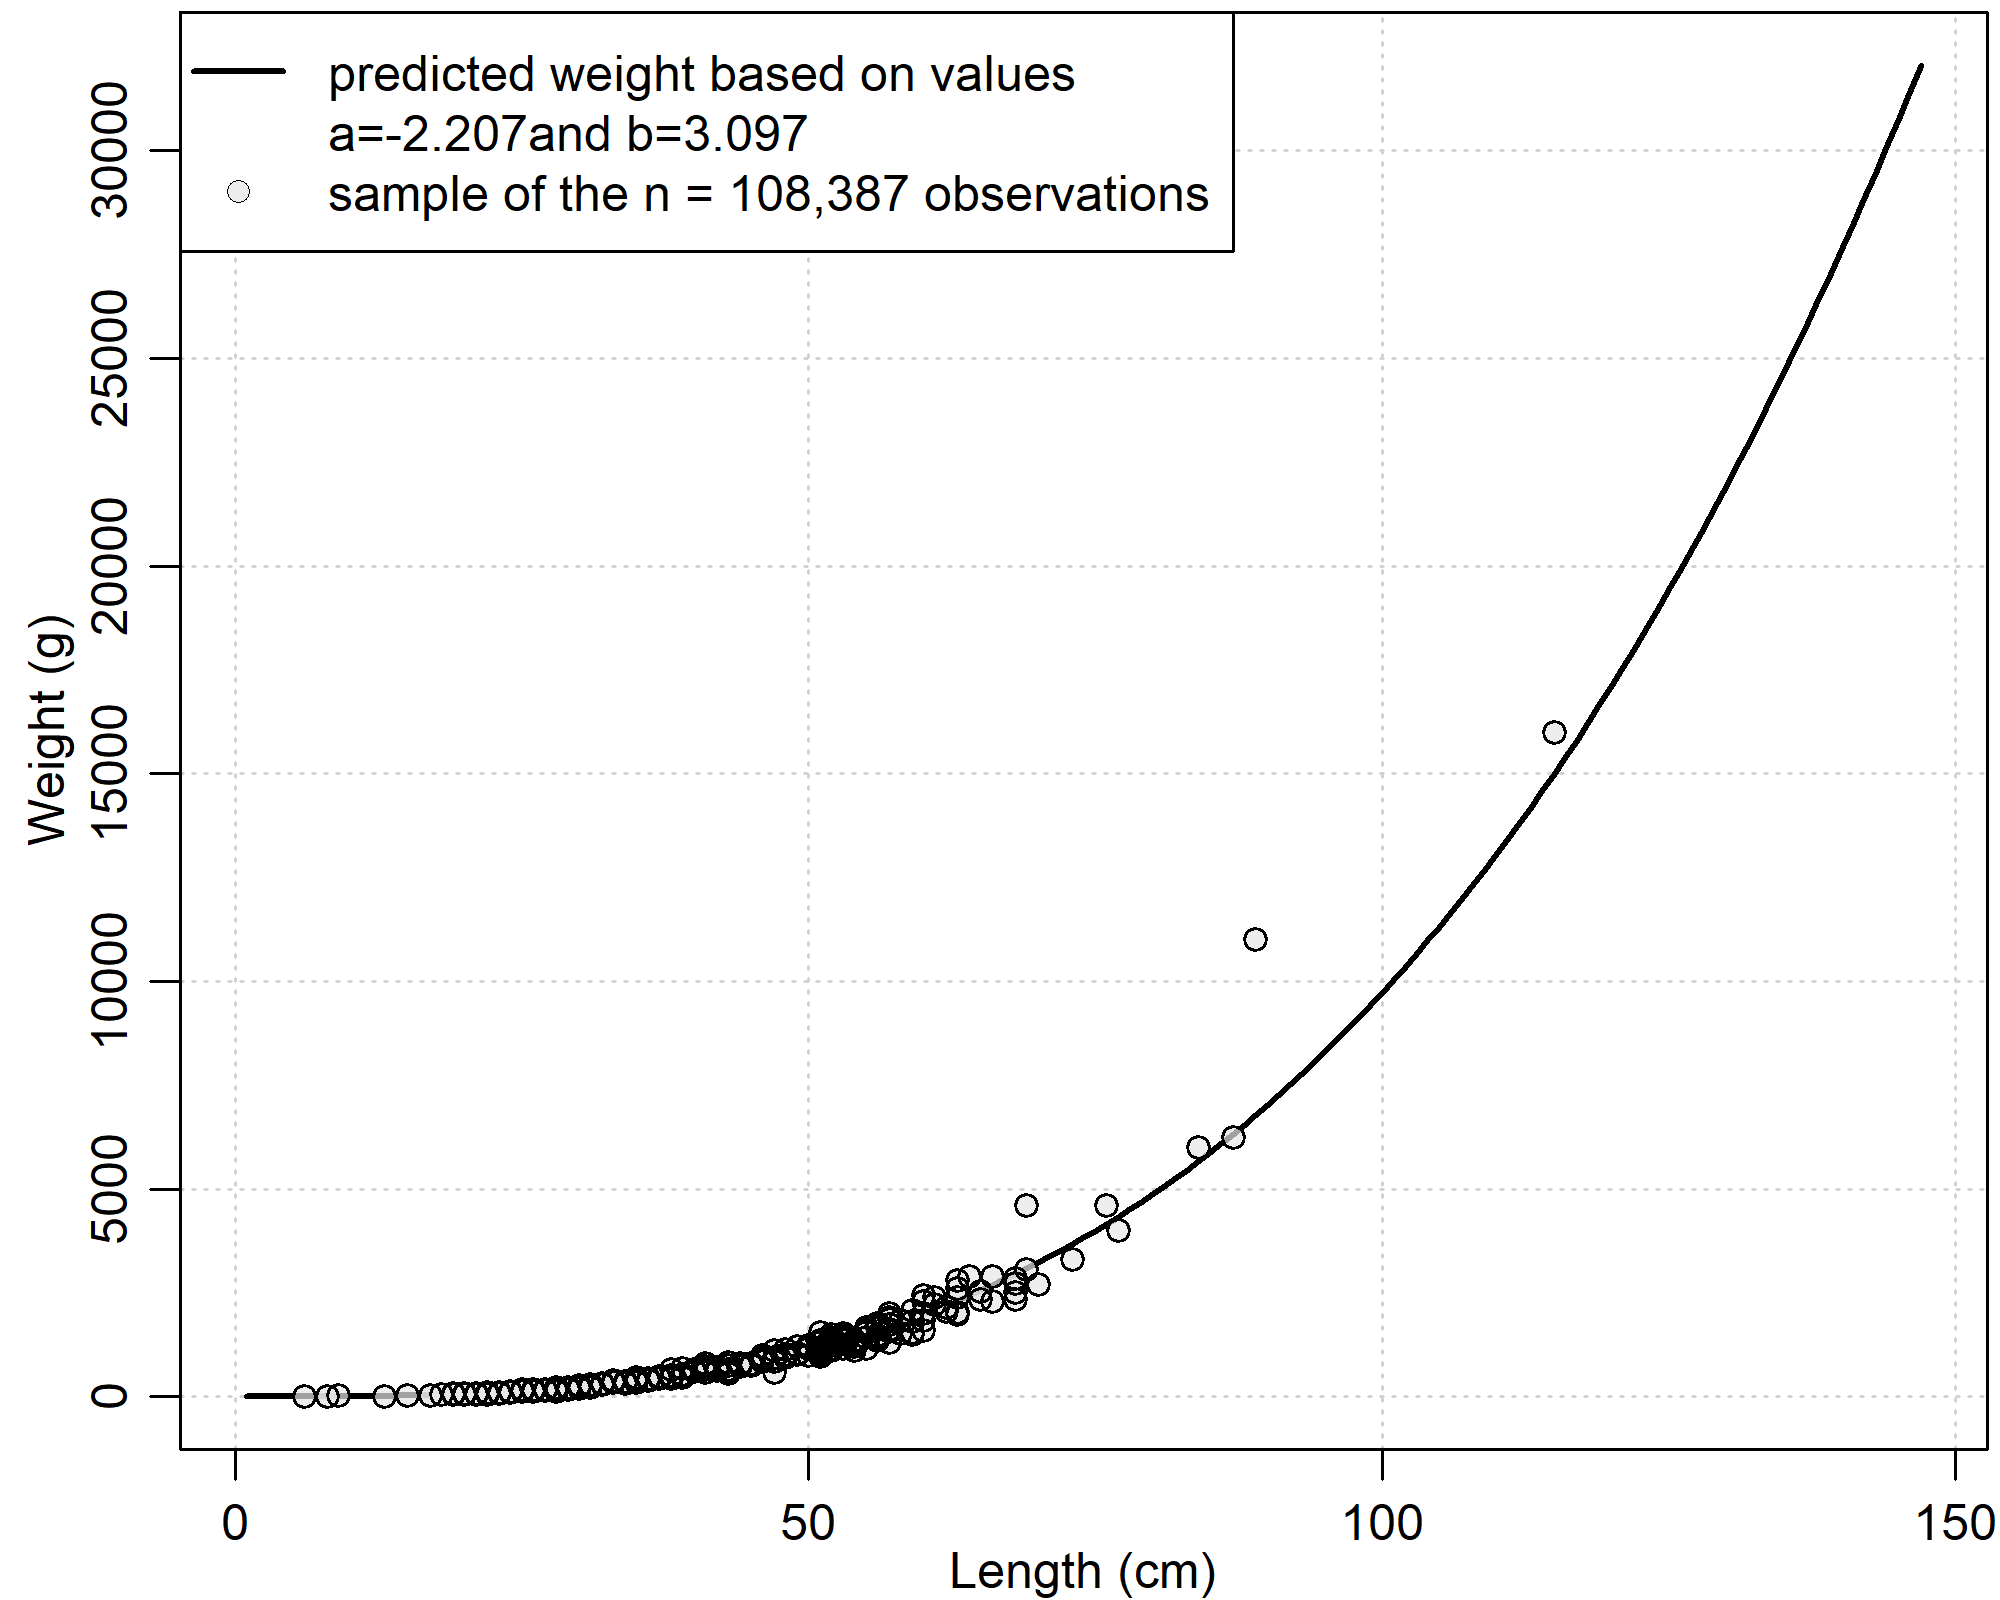
\includegraphics[width=6in]{./figure/LW-example}}{Figure \ref{fig:fig1}} 

}

\caption{Example of a length-weight relationship.}\label{fig:fig1}
\end{figure}
\clearpage

\clearpage

\hypertarget{references}{%
\section{References}\label{references}}

\noindent \vspace{-2em} \setlength{\parindent}{-0.2in} \setlength{\leftskip}{0.2in} \setlength{\parskip}{8pt}

\hypertarget{refs}{}
\begin{CSLReferences}{1}{0}
\leavevmode{\hypertarget{ref-Froese-etal-2014}{}}%
Froese, R., Thorson, J.T., and Reyes Jr, R.B. 2014. \link{https://doi.org/10.1111/jai.12299}{A bayesian approach for estimating length-weight relationships in fishes}. Journal of Applied Ichthyology 30(1): 78--85.

\leavevmode{\hypertarget{ref-Lai-Hesler-2004}{}}%
Lai, H.-L., and Helser, T. 2004. \link{https://doi.org/10.1016/j.fishres.2004.08.014}{Linear mixed-effects models for weight--length relationships}. Fisheries Research 70(2): 377--387.

\leavevmode{\hypertarget{ref-Ma-etal-2017}{}}%
Ma, Q., Y., J., and Ren, Y. 2017. \link{https://doi.org/10.1371/journal.pone.0171811}{Linear mixed-effects models to describe length-weight relationships for yellow croaker (\emph{{L}arimichthys polyactis}) along the north coast of china}. PLoS One.

\end{CSLReferences}
\end{document}
